\section{Game Design}

% Base on our pilot study results, we understand that if the cooperative game require High-Level Feature Communication, play it with non-common language player is really frustrating. According to GameFlow[1], games challenging should match the player’s skill level, If the challenges are greater than the skills, the result is anxiety and frustrating, if the challenges are less than the skills, the result is apathy and boring.

Based on our pilot study results, we realize that if playing cooperative games requires high-level-feature communication, playing with non-common language players would feel deeply frustrated. According to GameFlow\cite{GD1}, game challenges should match the player's skill level. If the challenges are greater than the player's skills, the gameplay result will be anxiety and frustrating. But, by constrast, if the challenges are less than the player's skills, the result will be apathy and boring.

% According to our observation, play cooperative game with different language speaker will significantly decrease cooperative skills which is really important for most cooperative games and the game challenge become too hard for this situation and causing frustrating. The most easy way to solve this problem is to decrease the game challenge difficulty for non-common language players, but it is not practical for commercial games because the players with common language would feel boring with no difficulty.

According to our observation, playing cooperative game with different language speaker will significantly decrease cooperative skills which is really important for most cooperative games. And game challenges would become too hard for this situation and cause frustrated. The easiest way to solve this problem is to decrease the game's difficulty for non-common language players. Nevertheless, this method is not practical for commercial games because it will make players with common language feel boring with no difficulty while playing the game.  

\begin{figure}[!h]
\centering
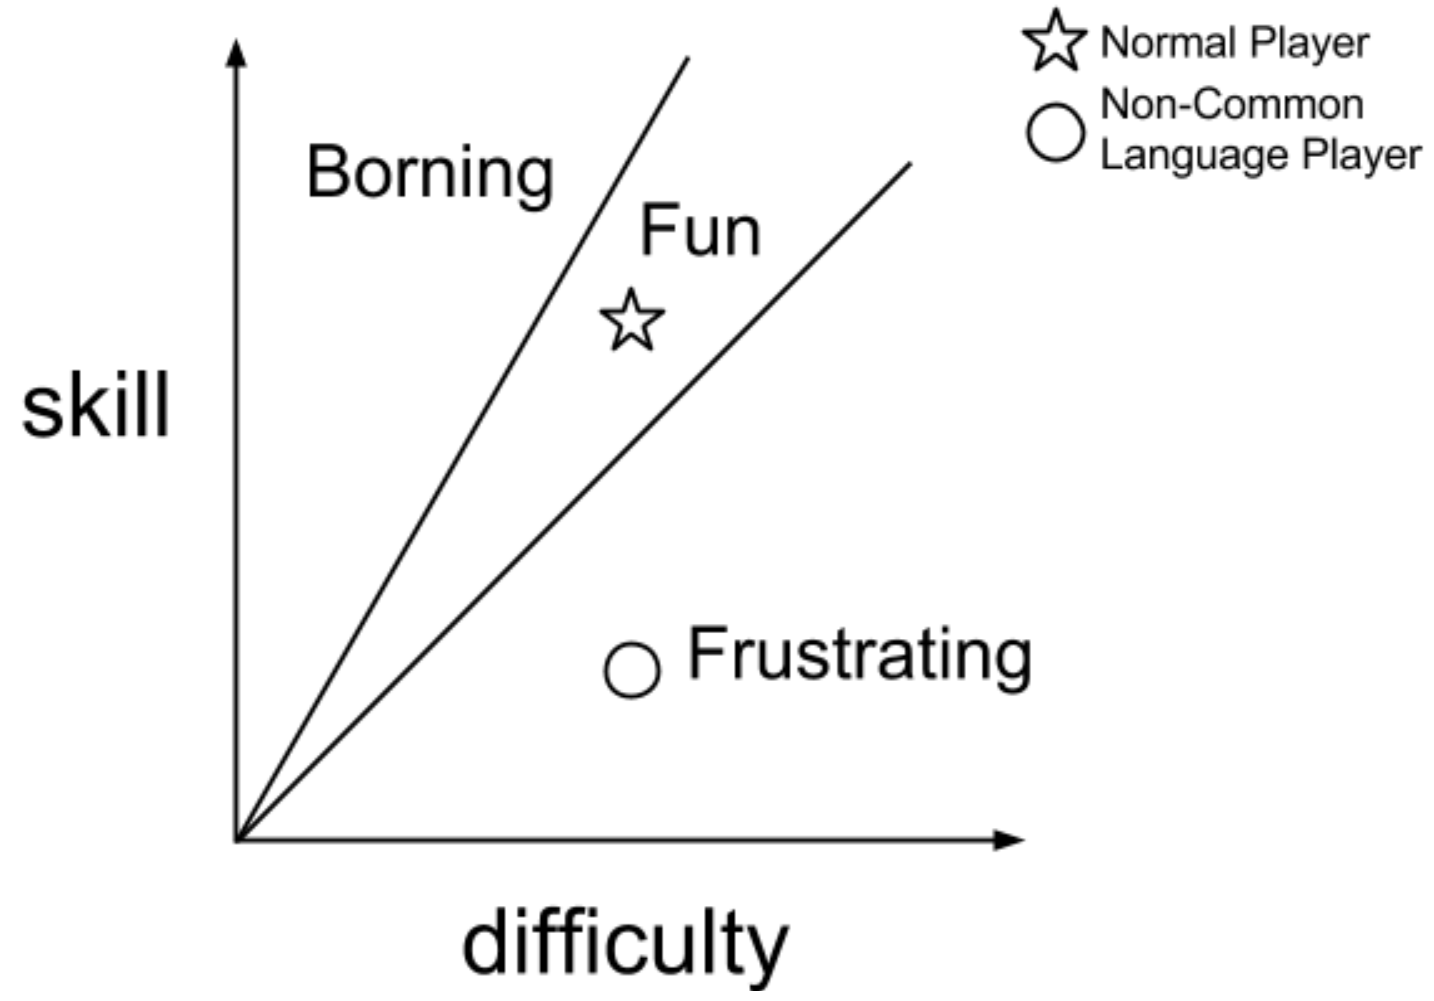
\includegraphics[width=0.9\columnwidth]{Figures/GD_F1.png}
\caption{Language boundary is causing player's skill difference}
\label{fig:GD_F1}
\end{figure}

\subsection{Body Language}
hi
\subsection{Prototype-Mute Robot}
hi
\subsection{Level Design}
hi
\subsection{System Implementation}
hi